\chapter{机器人探索算法和调度策略}

\section{机器人和探索空间}


\subsection{探索空间定义}
离散模型中,探索空间一般抽象为一个无向连通图,图的每个结点代表空间上机器人可达的位置,边代表机器人可以通过的路径,机器人沿着该路径到达相邻的空间位置。空间中每个位置结点在同一个时间至多只有一个机器人。

\begin{figure}[!hbt]
	\centering
	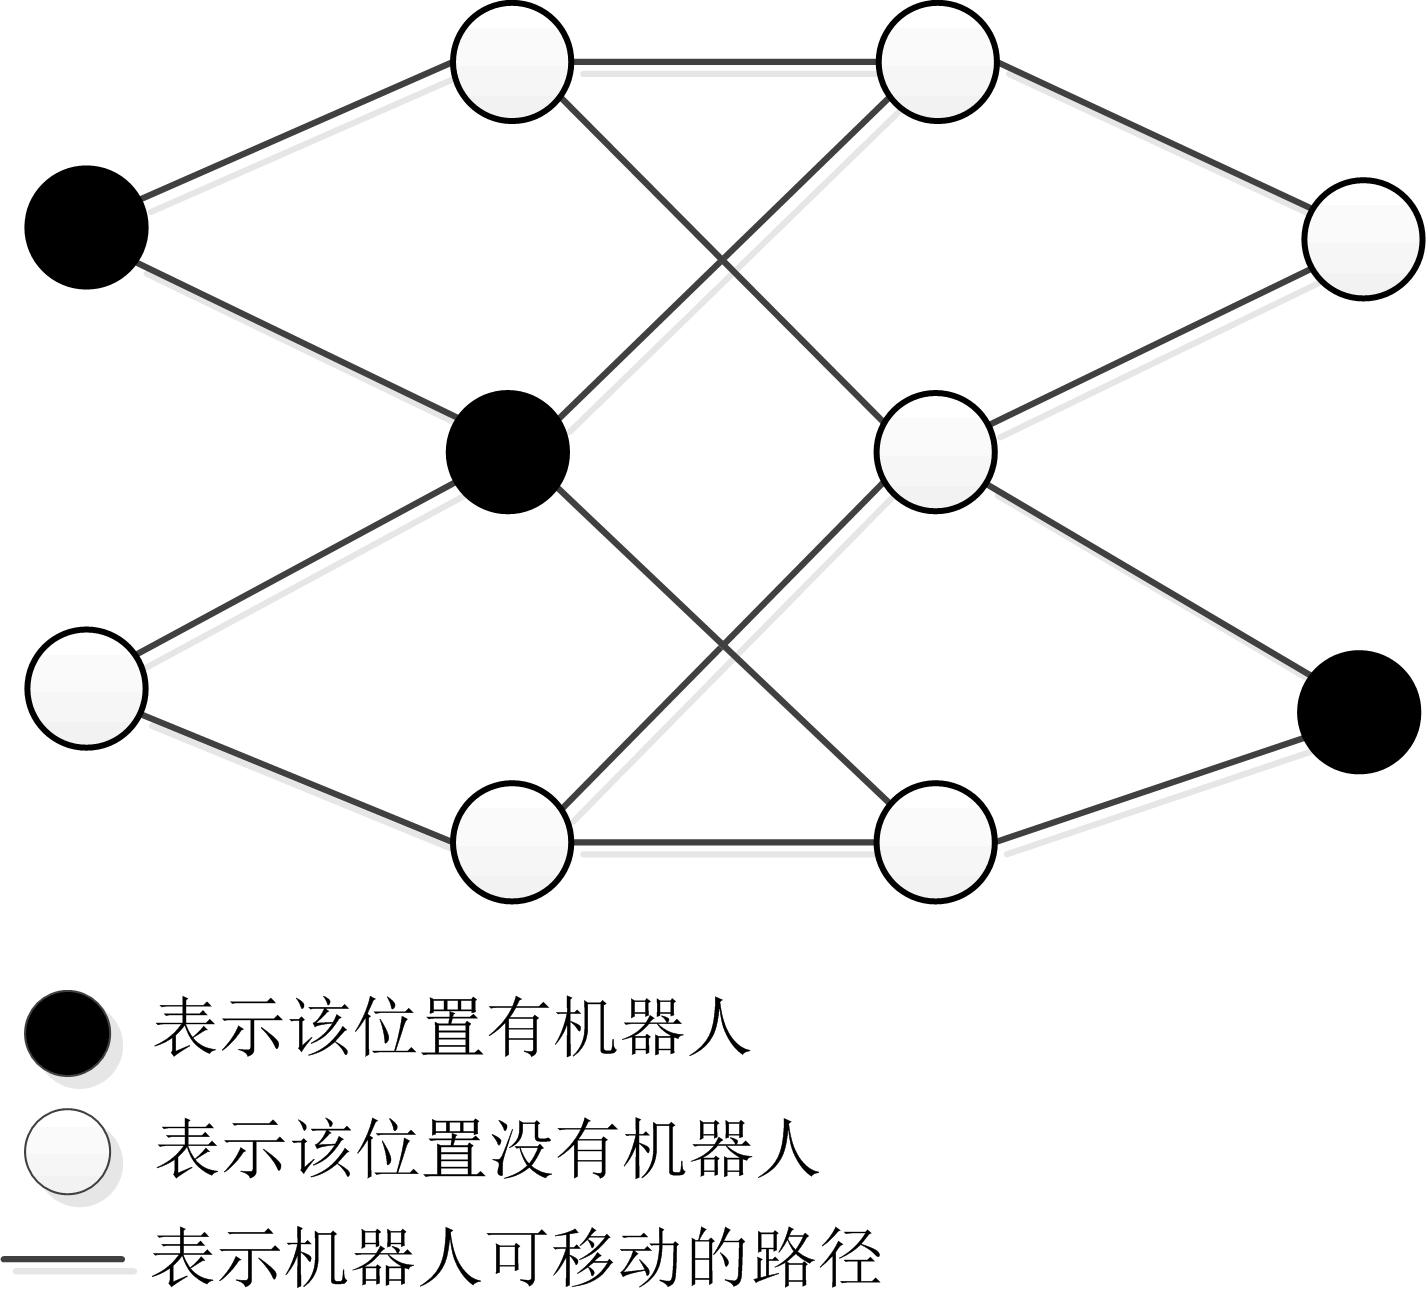
\includegraphics[width=3 in]{fig/normalspace.png}
	\caption{无向连通图表示探索空间}
	\label{fig:normalspace}
\end{figure}

如图\ref{fig:normalspace}给出了一个简单的离散探索空间的无向连通图表示,黑色结点表示该空间位置在此刻有一个机器人,白色结点说明该空间位置上没有机器人,图中有三个机器人,分别位于三个黑色的空间结点上。类似于计算机网络拓扑结构,探索空间结构也有总线拓扑结构、星型拓扑结构、环形拓扑结构、树形拓扑结构等。

\subsection{机器人移动三个阶段}
离散空间上每个机器人的移动分为三个阶段,分别是观察(look)、计算(compute)和移动(move).在观察阶段,机器人通过自身的视觉传感器,获取空间环境中其他机器人的位置快照信息。然后进入计算阶段,计算阶段根据观察阶段获取的位置快照信息,匹配自身预先设置的移动算法,计算得出下一步的移动策略。移动策略包括机器人是否移动,若是移动,则是沿着那条路径进行。移动阶段,机器人的动力装置按照计算阶段的所得移动决策作出对应的移动。

\begin{figure}[!hbt]
	\centering
	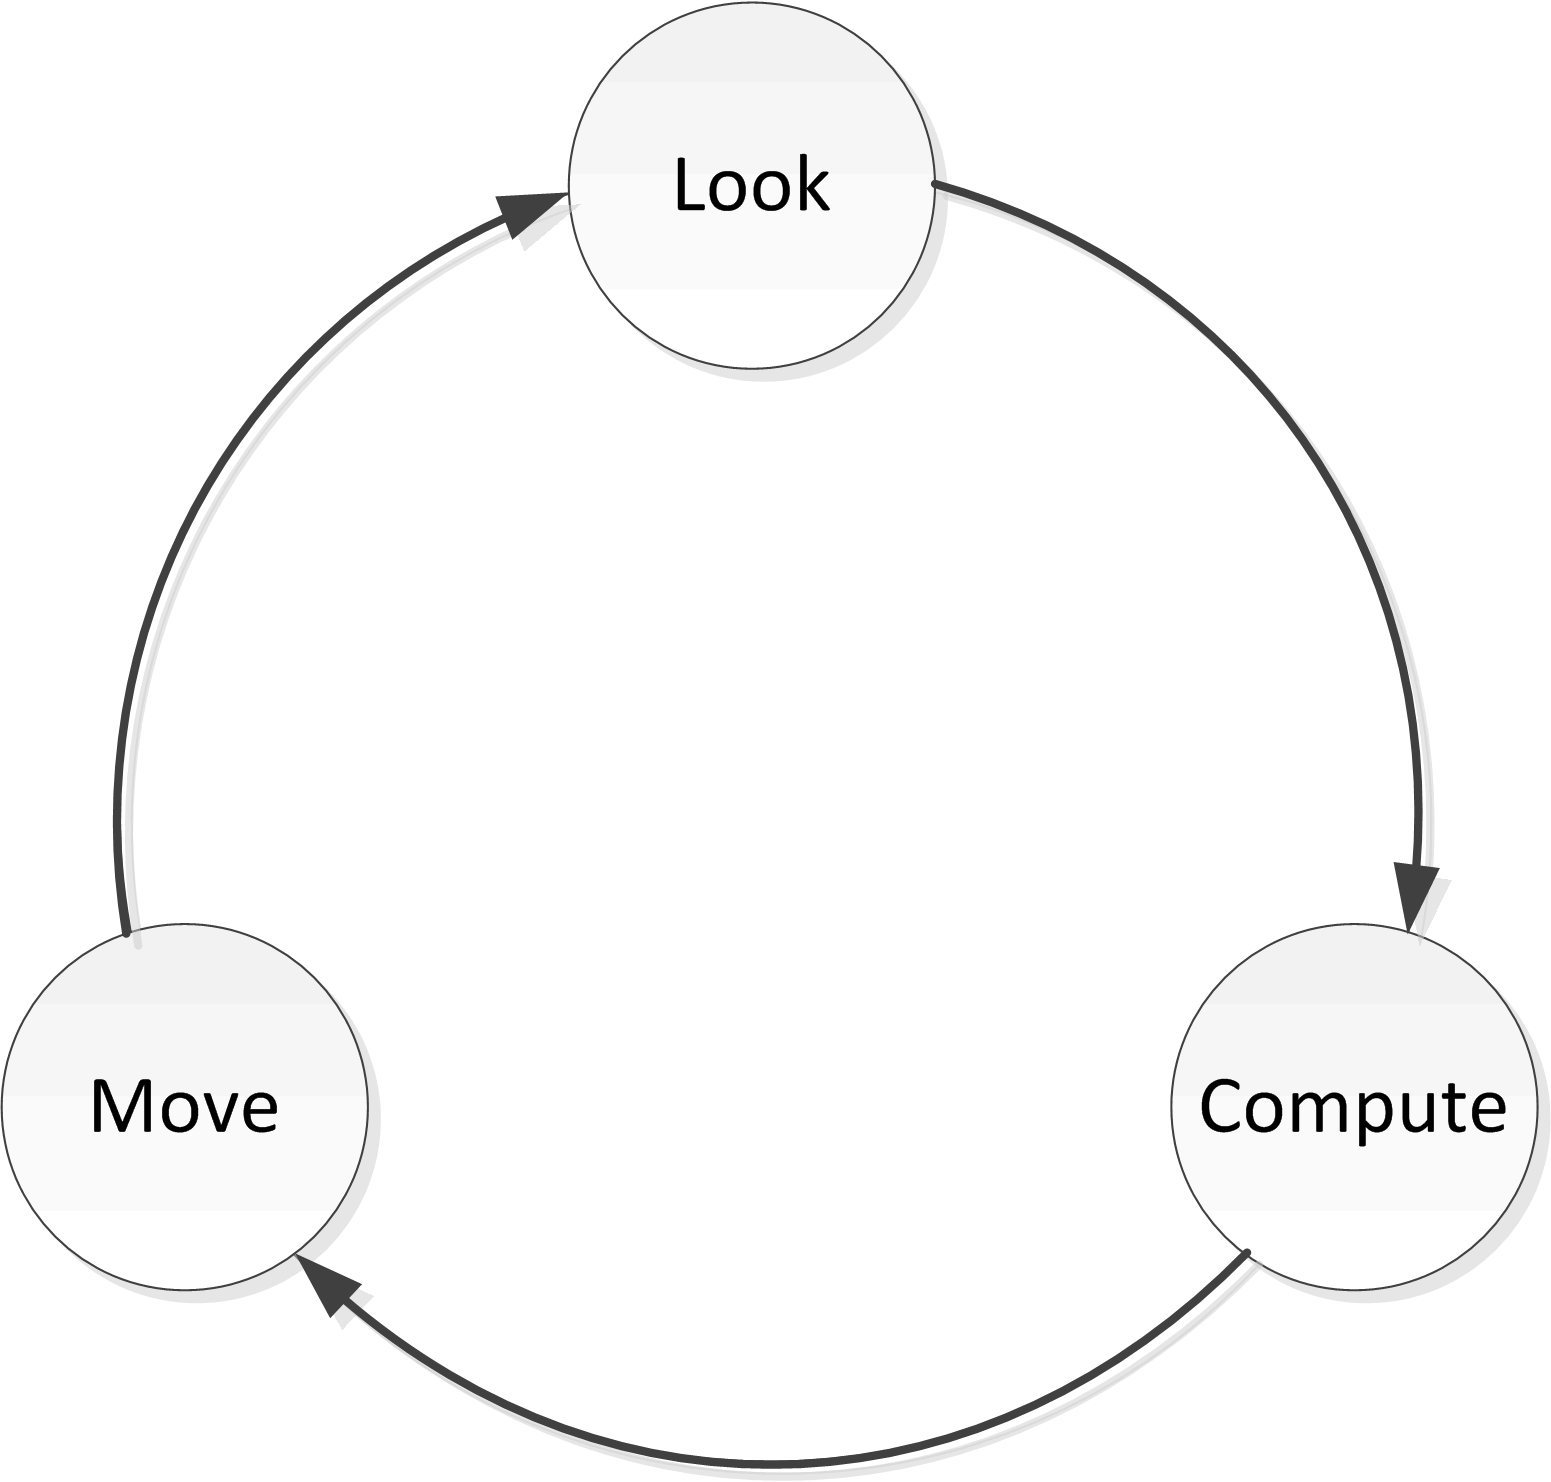
\includegraphics[width=3 in]{fig/robotthreephase.png}
	\caption{机器人移动三阶段}
	\label{fig:robotthreephase}
\end{figure}

如图\ref{fig:robotthreephase}描述了机器人移动的三个阶段,这三个阶段按照观察阶段、计算阶段、移动阶段,完成移动阶段之后又进入观察阶段,这样不断重复三个移动阶段。

\subsection{机器人移动调度模型}
原有模式中,Suzuki假设空间中机器人个数大于0,机器人的移动三个阶段具有原子性,且机器人之间的运动过程是同步的,提出了移动调度策略的两种变体,分别是完全同步调度模型FSYNC(fully-synchronous model)和半同步调度模型SSYNC(semi-synchronous model)。后来由Flocchini等人提出了异步调度模型ASYNC (asynchronous model),该异步调度模型中,机器人观察,计算,移动三个移动阶段不再具备原子性,这样可能会出现机器人使用过时的快照信息做出移动决策。

下面使用数学和算法知识来描述完全同步调度模型、半同步调度模型、异步调度模型具体的内容。

假设在一个离散空间中存在$k\left(k \in N^+ \right)$个机器人,使用集合$Rob =\left\{r_1,r_2,r_3,...,r_k\right\}$ 表示。空间位置结点可以按照一定顺序,对其进行编号,编号是空间位置结点的唯一标识,使用集合$Pos =\left\{n \in N^+ |0,1,2,...,n-1\right\}$ 表示空间所有空间位置结点,每个元素对应唯一一个空间位置结点。机器人是在空间位置结点上的,所以机器人与空间位置结点的映射关系使用$p:\left\{Rob \rightarrow Pos\right\}$表示,机器人r在某个时间所在图中的位置结点编号就为$p\left(r\right\) \in Pos \right)$。对于Rob 中的任意两个机器人$r_i,r_j\left(i \neq j \right)$,在任意一个时刻满足位置结点不相同$p\left(r_i\right) \neq p\left(r_j\right)$,即空间中任意时刻一个位子结点上至多只有一个机器人。

前面使用数学中的集合和映射定义了探索的离散空间、机器人已经机器人在空间结点上的函数关系,在此基础上,下面将介绍机器人移动的三种调度模型。完全同步调度模型是半同步调度模型的一种特殊情况,所以先介绍半同步调度模型,在介绍完全同步调度模型。完全异步调度模型完全与前面两种调度模型由较大区别,所以放在最后介绍。

将机器人移动的一个完整的观察、计算、移动称为完整移动阶段,在半同步调度模型中,Rob集合中只有选中的机器人才进行完整移动阶段。而半同步调度模型所有机器人都是同步而且观察、计算、移动都是具备原子性,所以可以每次选中的机器人是一个非空集合$Sched  \subseteq Rob $,在一个完整移动阶段开始之前,只有选入集合Sched的机器人才会执行完整移动阶段,即$\forall r \in Sched$执行观察、计算、移动,而$\forall r \notin Sched  $不执行。等到下一个完整移动阶段之前,又会从Rob随机选择一个机器人$Sched  \subseteq Rob $,重复上述过程。这就是半同步调度模型机器人调度的性质。下面使用简易算法过程,详细描述一下半同步调度模型中机器人执行完整移动阶段的过程。

\begin{lstlisting}
SSYNC-SCHEDULE(Rob)
  while
    choose Sched from Rob
    synchronous {
       foreach r in Sched{
          r.look
          r.compute
          r.move
       }
    }
\end{lstlisting}

半同步调度模型SSYNC-SCHEDULE的传入参数是机器人集合Rob,首先从Rob集合中选择子集合Sched且$Sched \neq \emptyset$。关键字\verb|synchronous|表示同步块中所有机器人同步完成移动阶段。在Sched 集合中的每个机器人开始同步执行观察、计算、移动。完成之后,又重新开始随机选择子集合Sched,重复不断执行上述过程。

完全同步调度模型是半同步调度模型中一种很特殊的情况,每次随机选择的集合$Sched = Rob $,即每次完整移动阶段之前在集合Rob中所有的机器人都被选中。使用算法过程描述如下:

\begin{lstlisting}
FSYNC-SCHEDULE(Rob)
  while
    synchronous {
       foreach r in Sched{
          r.look
          r.compute
          r.move
       }
    }
\end{lstlisting}

同半同步调度模型相对较而言,完全同步调度模型只是在每次选择集合$Sched$有所不同,其他过成完全相同。

而完全异步调度模型中,所有的机器人观察、计算、移动都是异步,没有原子性。类似于计算机系统的多线程,每个机器人的移动都是并行且互相之间没有同步约束,当一个机器人在观察时,其他机器人可能在执行计算或者移动。每个机器人执行移动的快慢完全是随机的,所以肯能会出现机器人在观察阶段通过视觉传感器获得快照是过时的。

\begin{lstlisting}
ASYNC-SCHEDULE(Rob)
    asynchronous {
       foreach r in Rob{
           while{
              r.look
              r.compute
              r.move
           }
       }
    }
\end{lstlisting}

上述完全异步调度模型算法中,关键字\verb|synchronous|表示Rob中所有的机器人都异步执行移动,对于每个机器人而言,都是在按照顺序不断重复执行观察、计算和移动过程,即整个过程中机器人都是并行执行完整移动阶段。

\section{环形空间探索算法}
探索空间结构有总线拓扑结构、星型拓扑结构、环形拓扑结构、树形拓扑结构,不同的探索空间结构有各自的特点,本文以环形拓扑结构空间为例.首先介绍环形拓扑结构环上的机器人视觉快照、匹配移动算法获取移动决策、移动决策的执行.在此基础上,将介绍永恒探索移动算法的相关概念.

\subsection{机器人视觉快照}
图\ref{fig:ring}给出一个简单的环形拓扑结构探索空间的例子。根据环形空间的自身特点,沿着环的顺时针方向,从\verb|0| 开始递增进行编号。所有位置编号组成的集合为Pos,图中黑色结点表示该位置结点上有机器人,白色结点表示该位置结点上没有机器人。下面给出某个时刻某个结点上机器人的数量的定义。

\begin{figure}[!hbt]
	\centering
	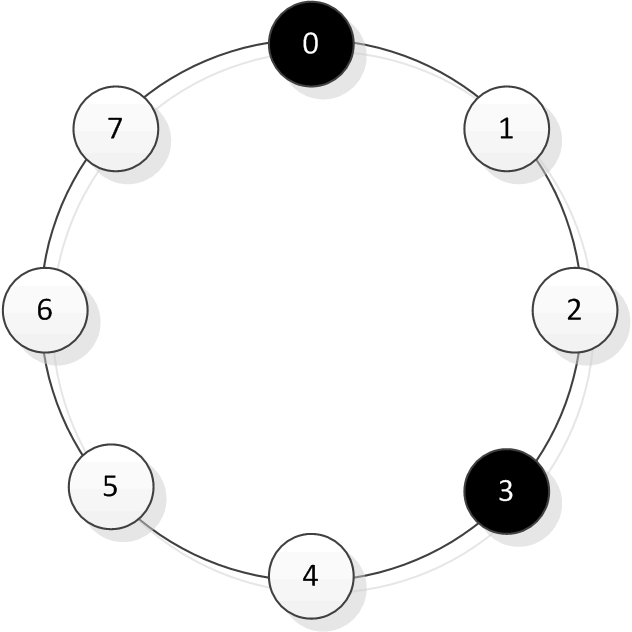
\includegraphics[width=2 in]{fig/ring.png}
	\caption{环形拓扑结构探索空间}
	\label{fig:ring}
\end{figure}

\begin{bfseries} 定义1\quad(结点机器人个数)\end{bfseries}结点机器人数$d_j$,\verb|j|表示结点的编号$j \in Pos $,当结点\verb|j|上有$k \left(k > 0\right)$机器人表示为$d_j = k$, 当结点\verb|j|没有机器人时,表示为$d_j = 0$。
\\

在环形拓扑结构的离散空间中,空间中的每个机器人可以顺时针观察,也可以逆时针观察。那么机器人每次观察的位置信息快照就有顺时针位置信息快照和逆时针位置信息快照两种,为了方便描述,给出某个位置上机器人获取位置信息快照的定义,如下:
\\

\begin{bfseries} 定义2\quad(机器人快照)\end{bfseries}离散空间上位置结点$p \in Pos$,\verb|j|上的机器人通过视觉传感器获取的位置快照为$\delta_p^F$,其中$F \in \left\{+,-\right\} $,\verb|+|表示顺时针,\verb|-|表示逆时针。
\\

在拥有\verb|n|个位置结点的环形拓扑结构的探索空间上,任意位置结点\verb|j|上机器人的顺时针和逆时针快照如下:

\verb|顺时针序列定义:| $\delta_p^+ = \left\langle d_j,d_{j+1},...,d_{j+n-1}  \right\rangle.$

\verb|逆时针序列定义:| $\delta_p^- = \left\langle d_j,d_{j-1},...,d_{j-n+1}  \right\rangle.$

如图\ref{fig:ring}中以位置编号为0的结点为例,其结点上机器人的顺时针和逆时针位置信息快照如下:

\verb|顺时针序列1:| $\delta_0^+ = \left\langle 1,0,0,1,0,0,0,0  \right\rangle.$

\verb|逆时针序列1:| $\delta_0^- = \left\langle 1,0,0,0,0,1,0,0  \right\rangle.$

虽然上述位置快照信息描述比较简洁和直观,但是当空间结点数n较大时,位置快照信息就过长,不利于描述。后来由lelia.blin在其文献[Ring]中提出了一种新的位置快照\verb|F-R|表达方式,\verb|F-R|表达方式中使用$F_m$表示连续的\verb|m|个空间位置结点上没有机器人,$R_n$表示连续的\verb|n|个空间位置结点上有机器人。那么顺时针序列1和逆时针序列1转化为F-R的表达方式为:

\verb|顺时针F-R序列1:| $\delta_0^+ = \left\langle R_1,F_2,R_1,F_4  \right\rangle.$

\verb|逆时针F-R序列1:| $\delta_0^- = \left\langle R_1,F_4,R_1,F_2   \right\rangle.$

F-R快照表达式中$F_m$和$R_n$的脚标值$m,n$都可以使用未知数表示,即可以限制$m,n$的取值范围,这样的表达十分灵活,描述性更强。

\subsection{机器人移动算法}






